\documentclass{beamer}
\usetheme{default}
\usepackage{graphicx}

\begin{document}
\begin{frame}{Angular correlation Function}
	$$F = 1 + a \frac{\boldsymbol{p_e}\cdot\boldsymbol{p_\nu}}{E_eE_\nu} + \frac{\boldsymbol{J}}J\cdot\left(A \frac{\boldsymbol{p_e}}{E_e} + B \frac{\boldsymbol{p_\nu}}{E_\nu} + D \frac{\boldsymbol{p_e}\times\boldsymbol{p_\nu}}{E_eE_\nu}\right)$$
	Spherical Coordinates ($\boldsymbol{J}$ parallel to positive Z axis)
	$$\boldsymbol{\beta_e} = (r=\beta_e;\theta=\theta_e;\phi=0),\;\cos(\theta_e) \equiv z_e,\;\beta_e = \frac{|\boldsymbol{p_e}|}{E} = \sqrt{1-\frac{m_e^2}{E^2}}$$
	$$\boldsymbol{\beta_\nu} = (r=1;\theta=\theta_\nu;\phi=\phi),\quad\cos(\theta_\nu) \equiv z_\nu$$
	$$\boldsymbol{\beta_e}\cdot\boldsymbol{\beta_\nu} = \beta_e(\cos\theta_e\cos\theta_\nu + \sin\theta_e\sin\theta_\nu\cos\phi) =$$
	$$ \beta_e(z_ez_\nu + \sqrt{1-z^2_e}\sqrt{1-z^2_\nu}\cos\phi)$$
	$$\boldsymbol{\beta_e}\cdot\boldsymbol{j} = \beta_e\cos\theta_e=\beta_ez_e$$
	$$\boldsymbol{\beta_\nu}\cdot\boldsymbol{j} = \cos\theta_\nu=z_\nu$$
	$$\boldsymbol{j}\cdot(\boldsymbol{\beta_e}\times\boldsymbol{\beta_\nu})=\beta_e\sin\theta_e\sin\theta_\nu\sin\phi=\beta_e\sqrt{1-z^2_e}\sqrt{1-z^2_\nu}\sin\phi$$
\end{frame}	
	
\begin{frame}{Single Variable: A}
	\begin{figure}
		\centering
		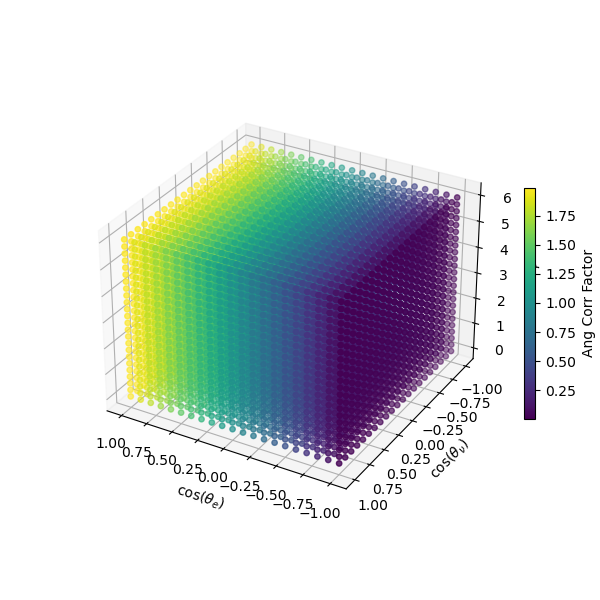
\includegraphics[width=0.4\paperwidth]{plots/A_3D_image.png}
		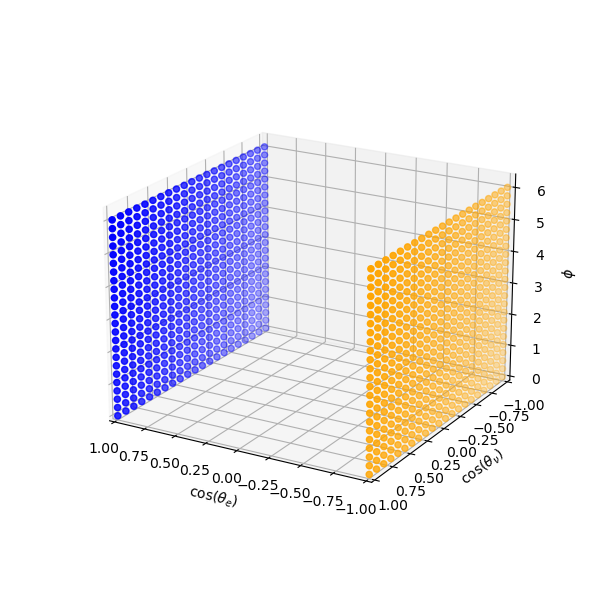
\includegraphics[width=0.4\paperwidth]{plots/A_max_min.png}
		\caption{(Right) Values of the angular correlation Factor with A = 1, E = 5000 keV and rest of variables 0. (Left) Location of maximum (blue, value = 1.995) and minimum (orange, value = 0.005)}
	\end{figure}
\end{frame}
\begin{frame}{Single Variable: A}
	\begin{figure}
		\centering
		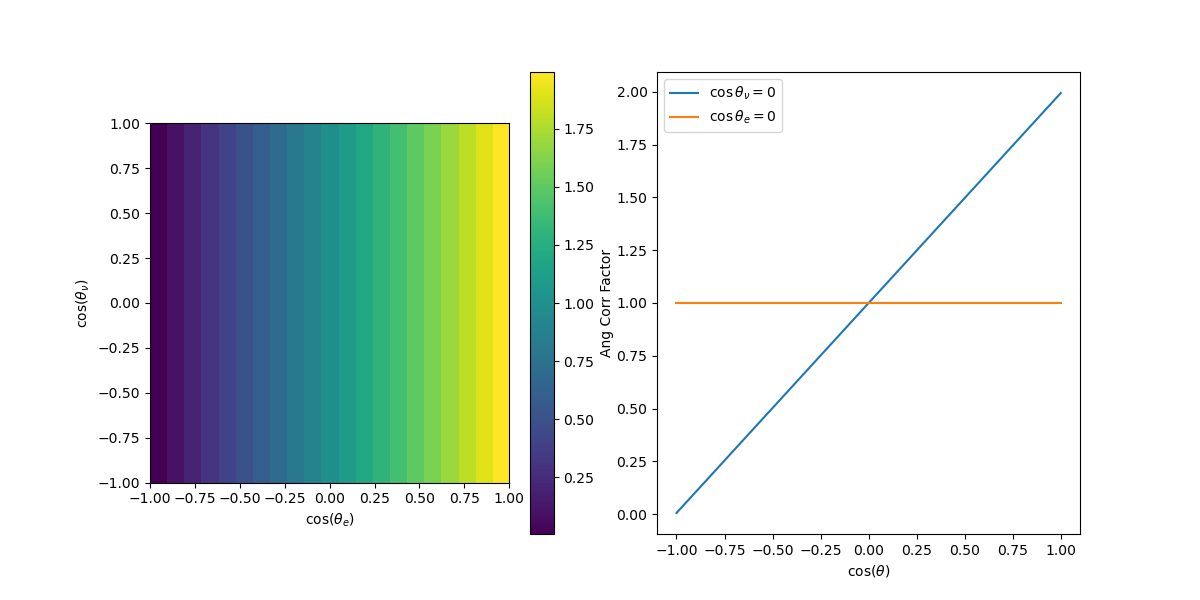
\includegraphics[width=0.8\paperwidth]{plots/crosssections_A.png}
		\caption{(Right) 2D projection of previous 3D image at any $\phi$ (Left) 1D projections at any $\phi$, and either $z_e = 0$ or $z_\nu = 0$ }
	\end{figure}
\end{frame}

\begin{frame}{Single Variable: B}
	\begin{figure}
		\centering
		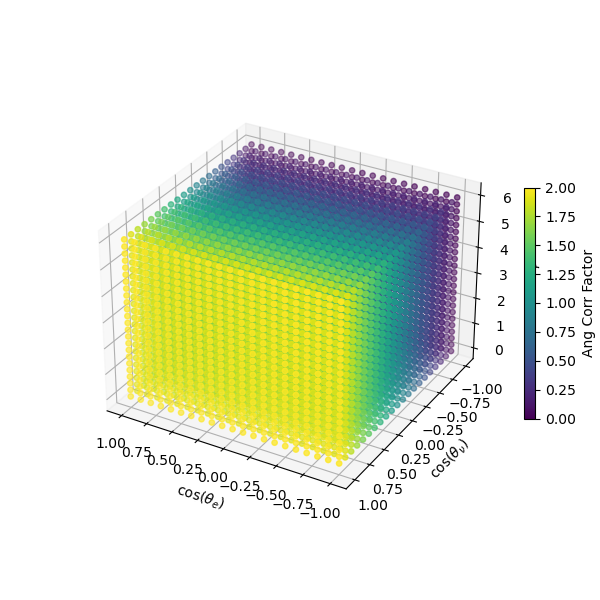
\includegraphics[width=0.4\paperwidth]{plots/B_3D_image.png}
		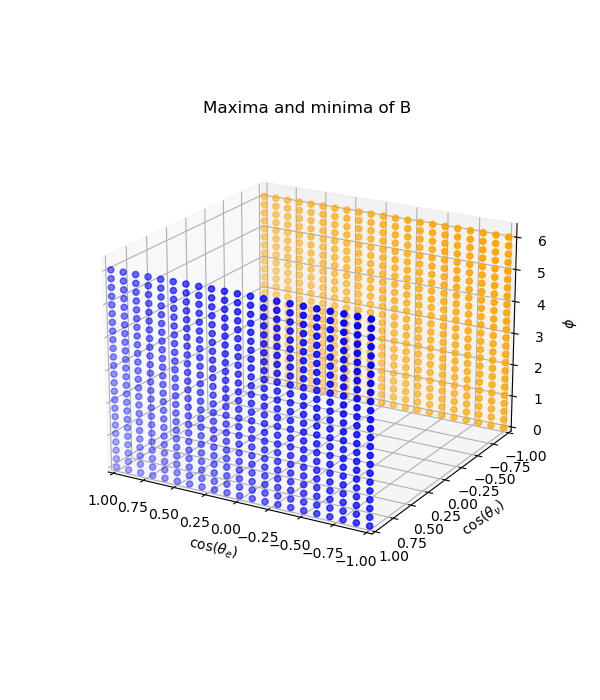
\includegraphics[width=0.4\paperwidth]{plots/B_max_min.png}
		\caption{(Right) Values of the angular correlation Factor with B = 1, E = 5000 keV and rest of variables 0. (Left) Location of maximum (blue, value = 2) and minimum (orange, value = 0)}
	\end{figure}
\end{frame}
\begin{frame}{Single Variable: B}
	\begin{figure}
		\centering
		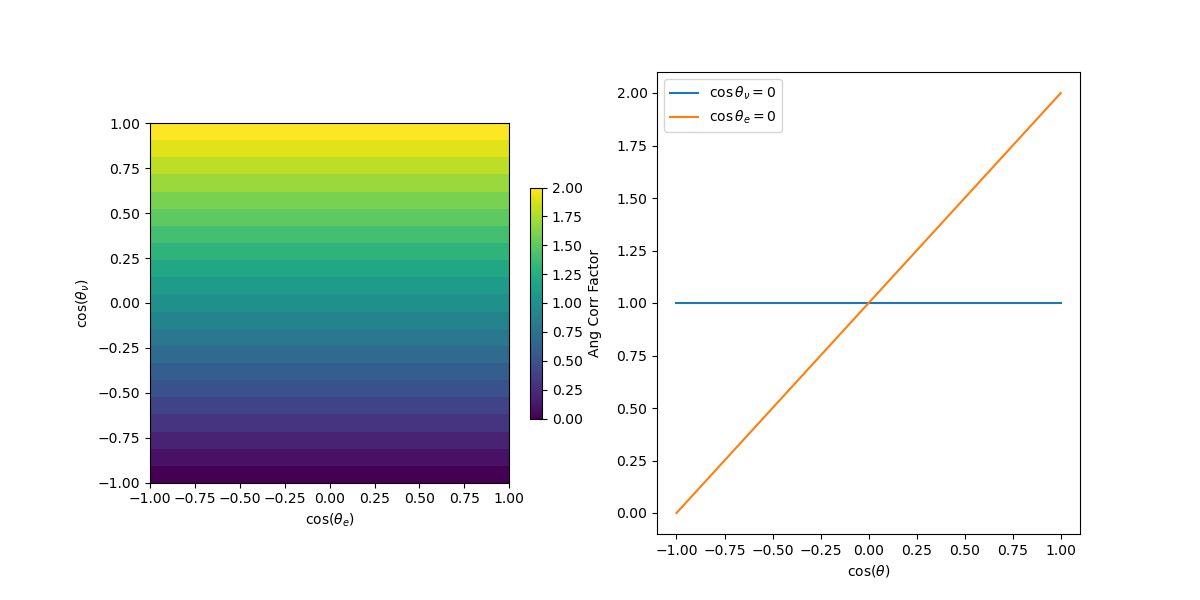
\includegraphics[width=0.8\paperwidth]{plots/crosssections_B.png}
		\caption{(Right) 2D projection of previous 3D image at any $\phi$ (Left) 1D projections at any $\phi$, and either $z_e = 0$ or $z_\nu = 0$ }
	\end{figure}
\end{frame}

\begin{frame}{Single Variable: a}
	\begin{figure}
		\centering
		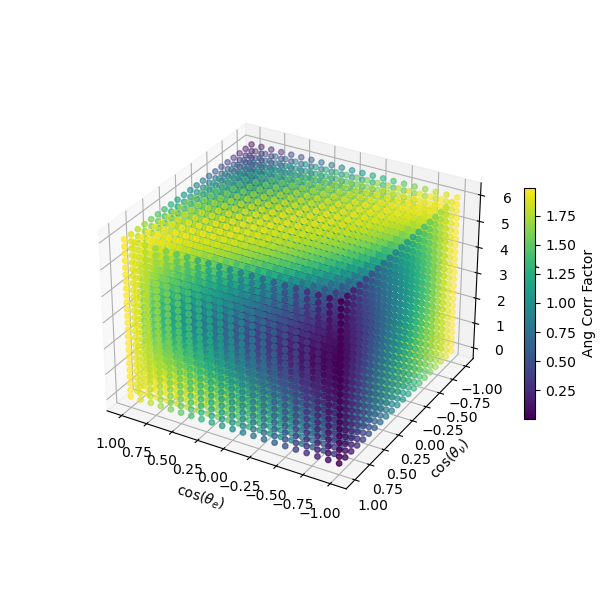
\includegraphics[width=0.4\paperwidth]{plots/a_3D_image.png}
		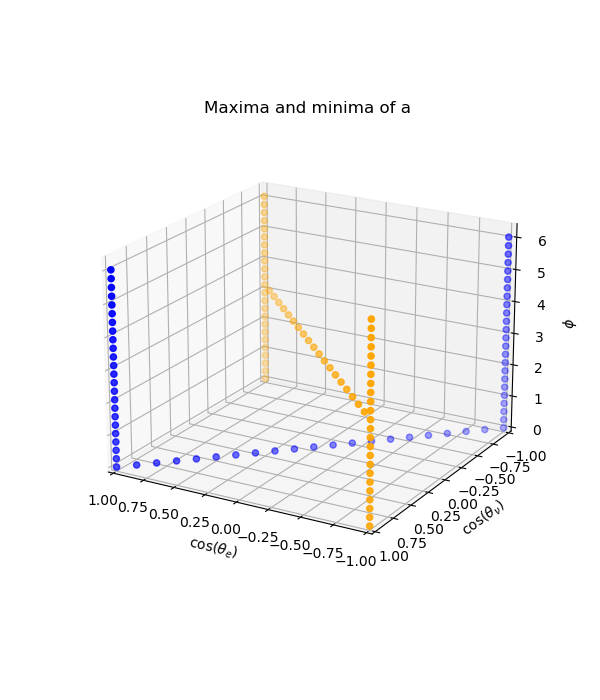
\includegraphics[width=0.4\paperwidth]{plots/a_max_min.png}
		\caption{(Right) Values of the angular correlation Factor with a = 1, E = 5000 keV and rest of variables 0. (Left) Location of maximum (blue, value = 1.995) and minimum (orange, value = 0.005)}	
	\end{figure}
\end{frame}
\begin{frame}{Single Variable: a}
	\begin{figure}
		\centering
		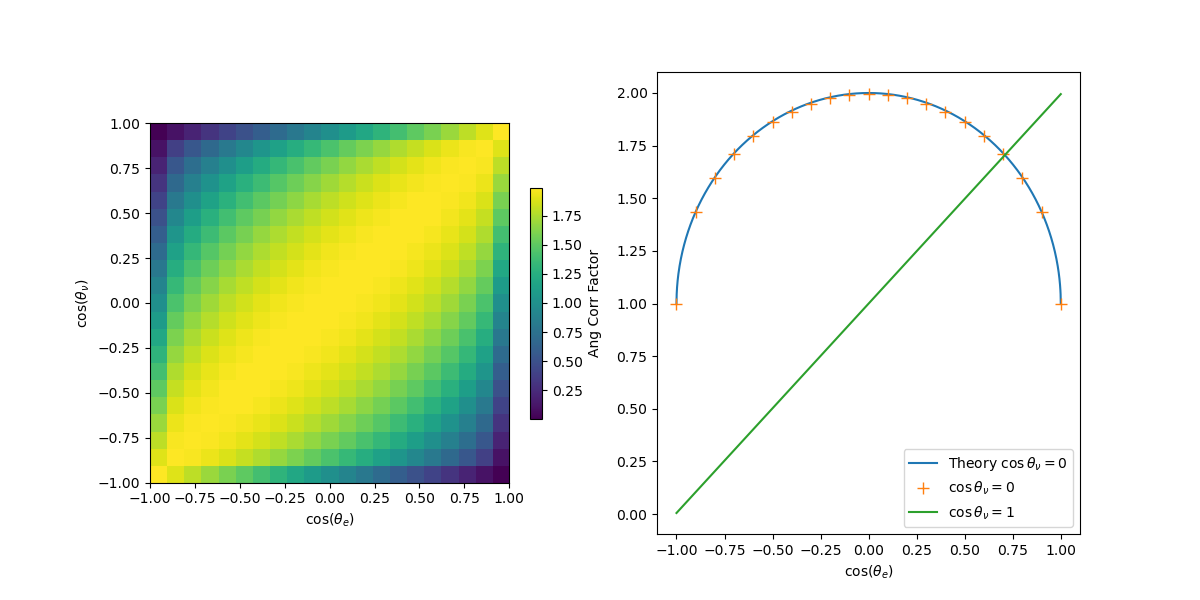
\includegraphics[width=0.8\paperwidth]{plots/crosssections_a.png}
		\caption{(Right) 2D projection of previous 3D image at $\phi = 0$ (Left) 1D projections at $\phi=0$, and either $z_\nu = 0$ or $z_\nu = 1$ }
	\end{figure}
\end{frame}

\begin{frame}{Single Variable: D}
	\begin{figure}
		\centering
		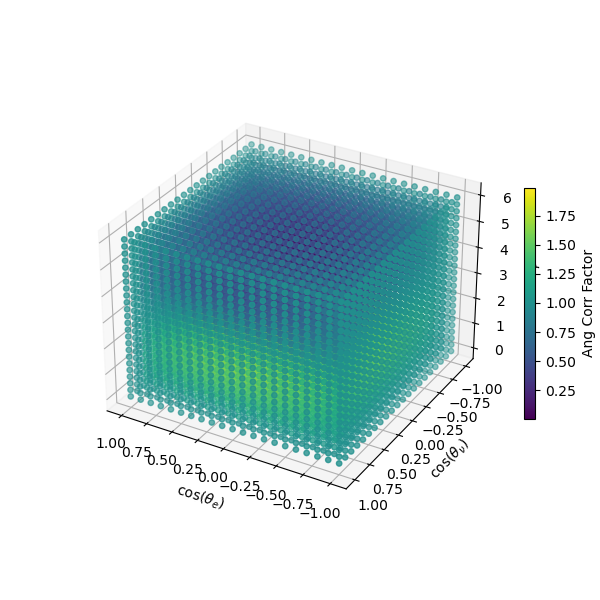
\includegraphics[width=0.4\paperwidth]{plots/D_3D_image.png}
		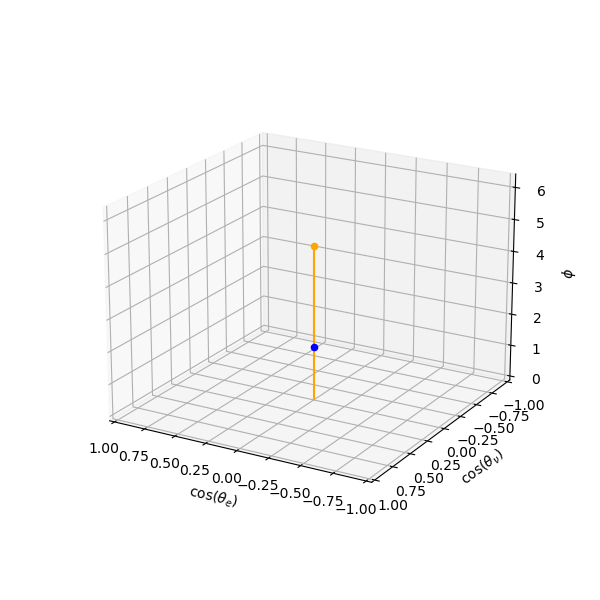
\includegraphics[width=0.4\paperwidth]{plots/D_max_min.png}
		\caption{(Right) Values of the angular correlation Factor with D = 1, E = 5000 keV and rest of variables 0. (Left) Location of maximum (blue, value = 1.995) and minimum (orange, value = 0.005)}	
	\end{figure}
\end{frame}
\begin{frame}{Single Variable: D}
	\begin{figure}
		\centering
		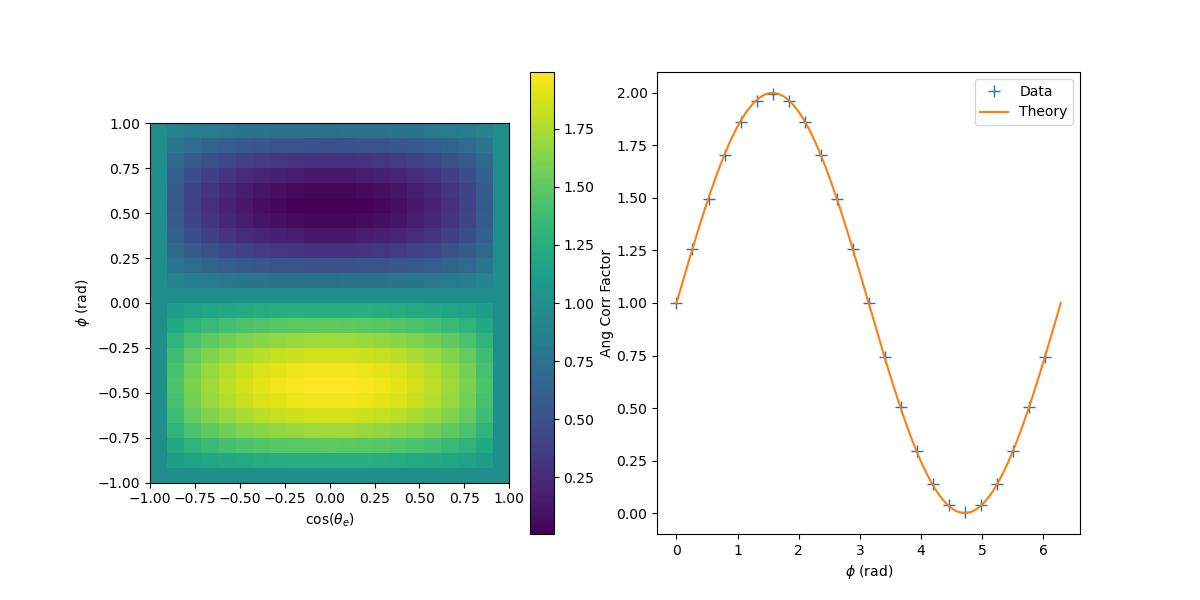
\includegraphics[width=0.8\paperwidth]{plots/crosssections_D.png}
		\caption{(Right) 2D projection of previous 3D image at $z_\nu = 0$ (Left) 1D projection at $z_\nu = 0$ and $z_\nu = 0$ }
	\end{figure}
\end{frame}
\begin{frame}{Two variables: A and B}
	Consider different ratios by either:
	\begin{itemize}
		\item Fixing $A = B = 1$ and modifying the energy (first 3 plots)
		\item Same as before, but now $B = -1$
		\item Fixing $B = 1$ and $E \gg m_e \rightarrow \beta_e \approx 1$ and modifying $A > B$
	\end{itemize}
		
	$$F = 1 + A\beta_ez_e + Bz_\nu$$
		
	No $\phi$ dependence: we can work in a 2D crosssection and capture all of the details.
	
\end{frame}
\begin{frame}{Two variables: A and B}{Low Energy, Positive B}
	\begin{figure}
		\centering
		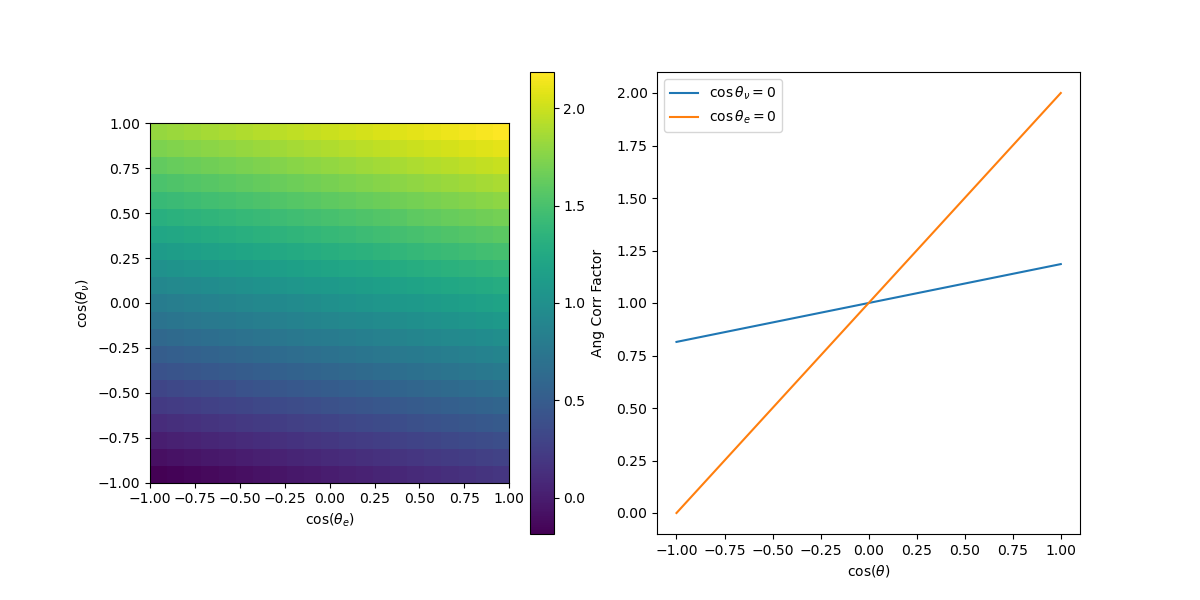
\includegraphics[width=0.8\paperwidth]{plots/posA_posB_lowE.png}
		\caption{(Right) Values of the angular correlation Factor with $A = B = 1$, $E = 520$ keV and rest of variables 0. Maximum = 2.18526, Minimum = -0.18526 (Left) 1D projections at any $\phi$, and either $z_e = 0$ (orange, slope $\equiv$ m = 1) or $z_\nu = 0$ (blue, m = 0.1852)}	
	\end{figure}
\end{frame}
\begin{frame}{Two variables: A and B}{Medium Energy, Positive B}
	\begin{figure}
		\centering
		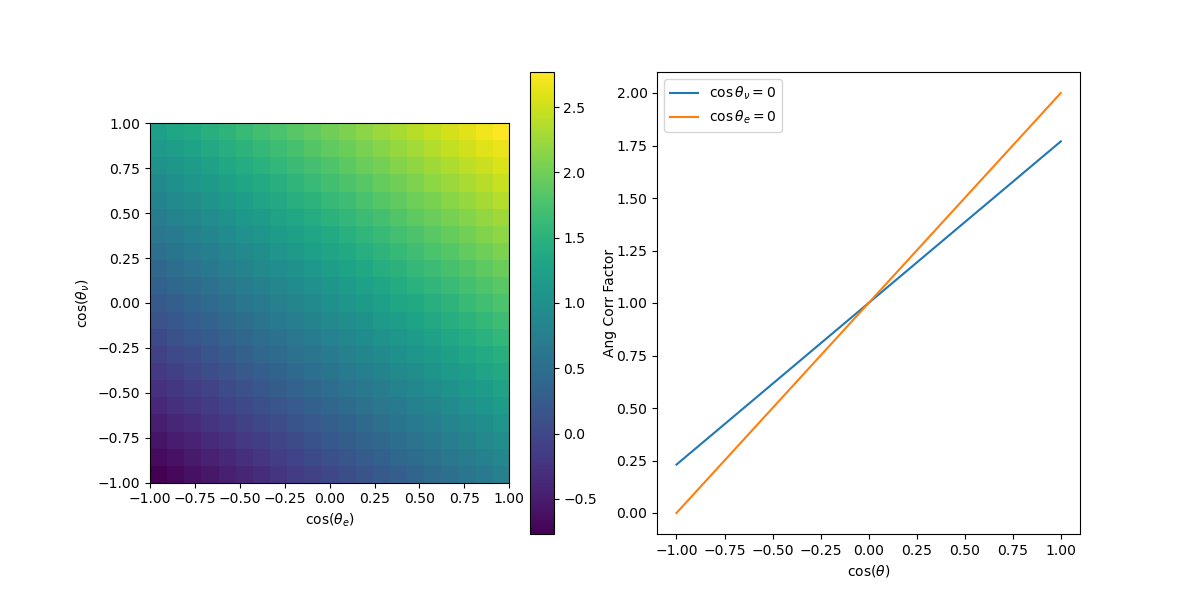
\includegraphics[width=0.8\paperwidth]{plots/posA_posB_medE.png}
		\caption{(Right) Values of the angular correlation Factor with $A = B = 1$, $E = 800$ keV and rest of variables 0. Maximum = 2.76942, Minimum = -0.76942 (Left) 1D projections at any $\phi$, and either $z_e = 0$ (orange, m = 1) or $z_\nu = 0$ (blue, m = 0.7694)}	
	\end{figure}
\end{frame}
\begin{frame}{Two variables: A and B}{High Energy, Positive B}
	\begin{figure}
		\centering
		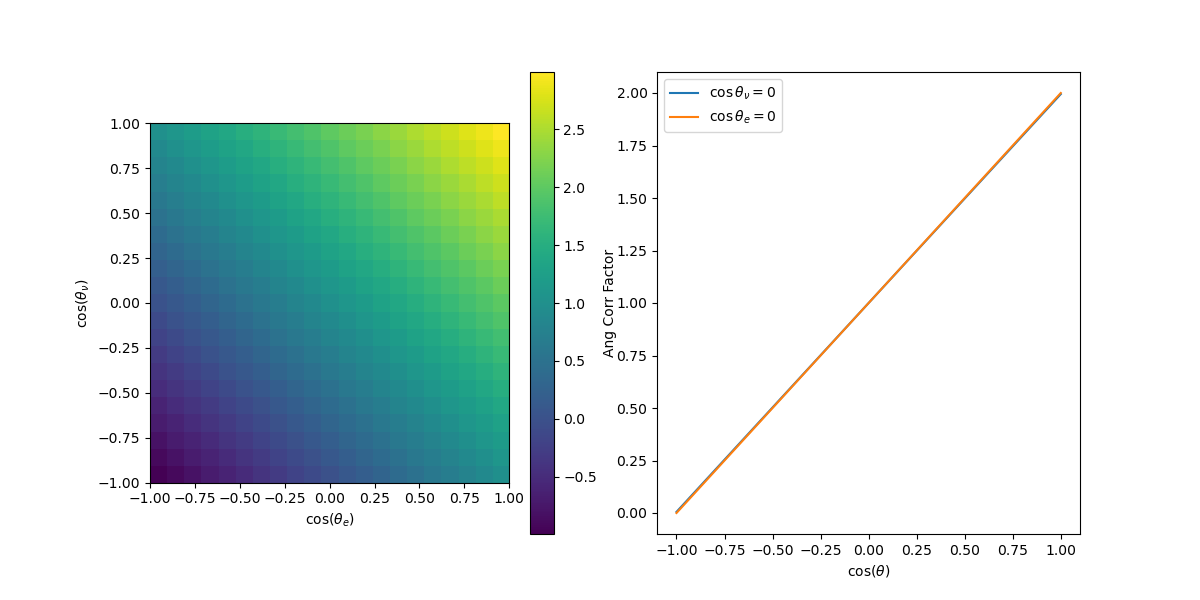
\includegraphics[width=0.8\paperwidth]{plots/posA_posB_hiE.png}
		\caption{(Right) Values of the angular correlation Factor with $A = B = 1$, $E = 5000$ keV and rest of variables 0. Maximum = 2.99476, Minimum = -0.99476 (Left) 1D projections at any $\phi$, and either $z_e = 0$ (orange, m = 1) or $z_\nu = 0$ (blue, m = 0.9948)}	
	\end{figure}
\end{frame}
\begin{frame}{Two variables: A and B}{High A, Positive B}
	\begin{figure}
		\centering
		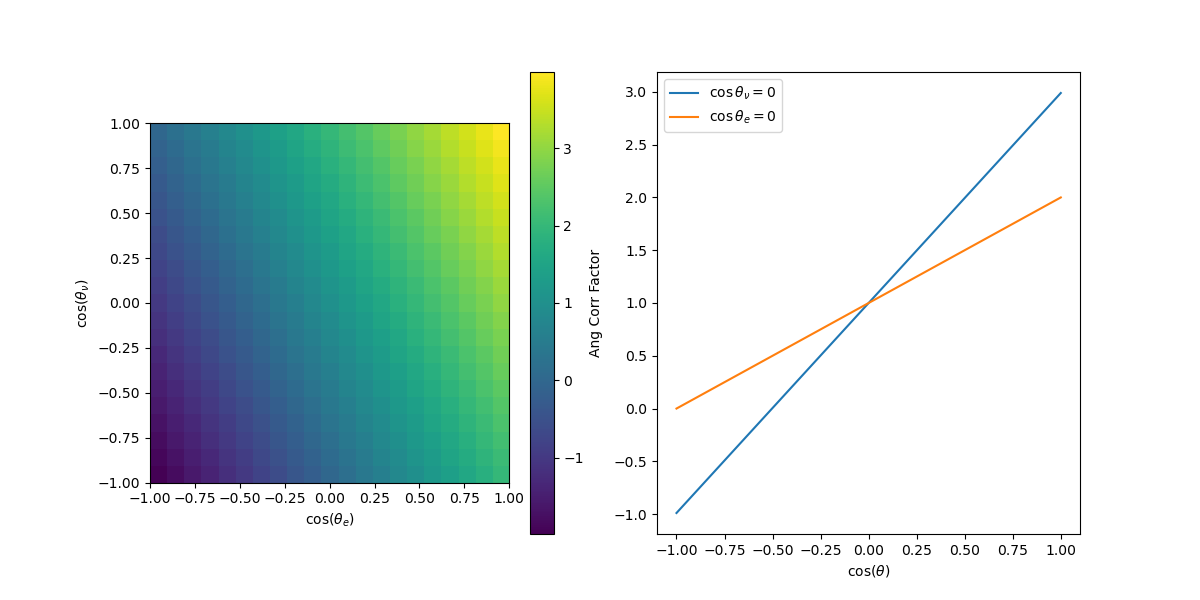
\includegraphics[width=0.8\paperwidth]{plots/posA_posB_hiA.png}
		\caption{(Right) Values of the angular correlation Factor with $A = 2$, $B = 1$, $E = 5000$ keV and rest of variables 0. Maximum = 3.98953, Minimum = -1.98953 (Left) 1D projections at any $\phi$, and either $z_e = 0$ (orange, m = 1) or $z_\nu = 0$ (blue, m = 1.9895)}	
	\end{figure}
\end{frame}
\begin{frame}{Two variables: A and B}{Very High A, Positive B}
	\begin{figure}
		\centering
		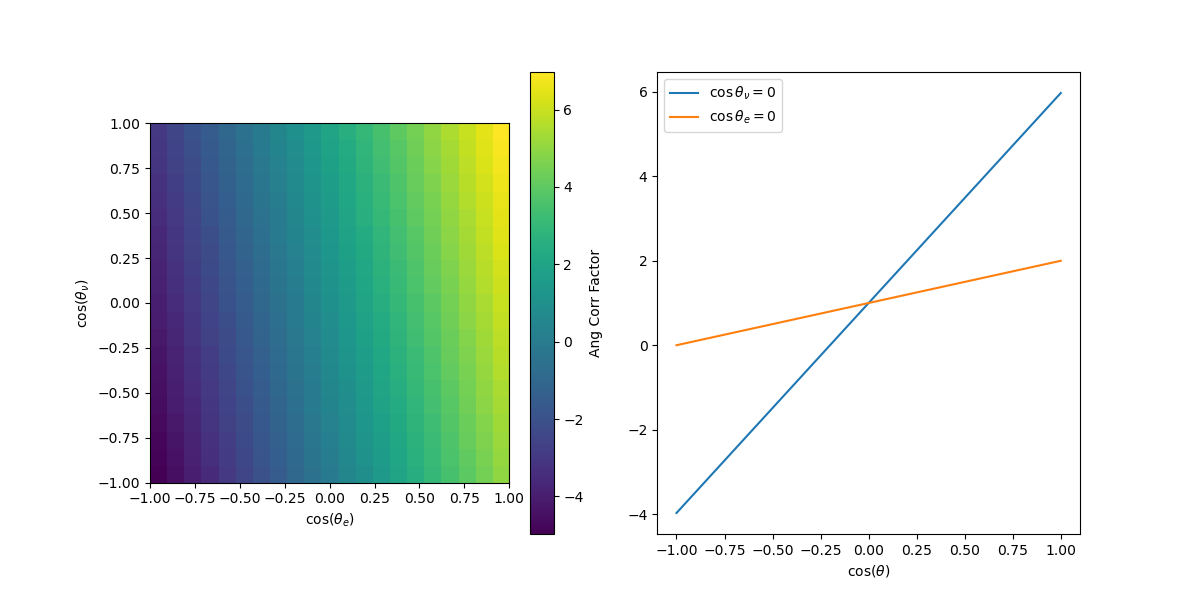
\includegraphics[width=0.8\paperwidth]{plots/posA_posB_vhiA.png}
		\caption{(Right) Values of the angular correlation Factor with $A = 5$, $B = 1$, $E = 5000$ keV and rest of variables 0. Maximum = 3.98953, Minimum = -1.98953 (Left) 1D projections at any $\phi$, and either $z_e = 0$ (orange, m = 1) or $z_\nu = 0$ (blue, m = 1.9895)}	
	\end{figure}
\end{frame}
\begin{frame}{Two variables: A and B}{Low Energy, Negative B}
	\begin{figure}
		\centering
		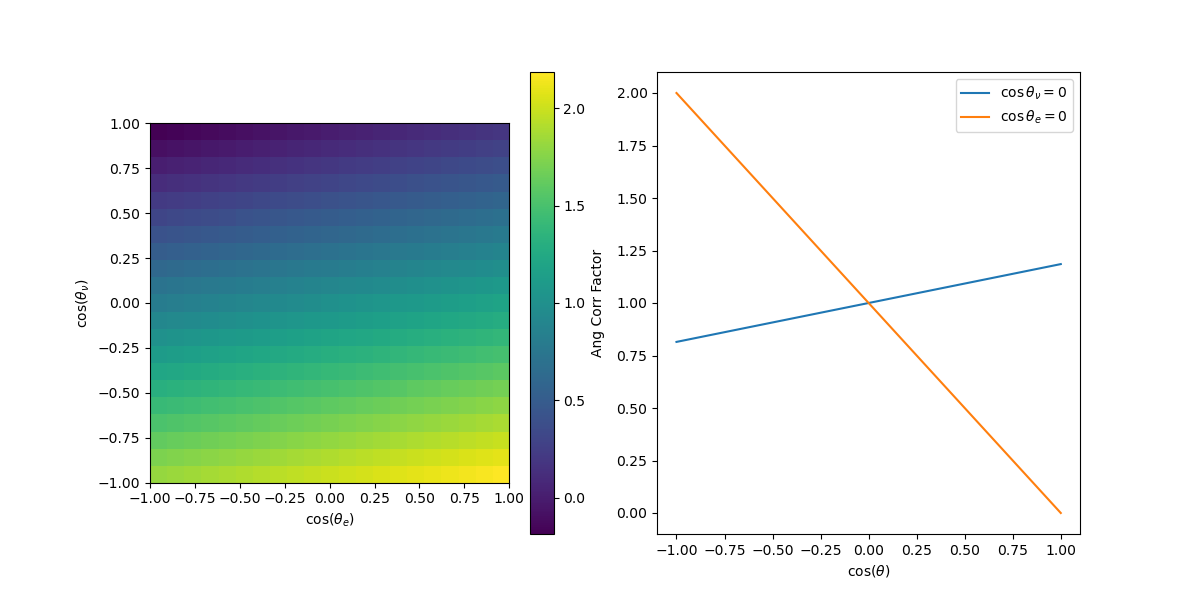
\includegraphics[width=0.8\paperwidth]{plots/posA_negB_lowE.png}
		\caption{(Right) Values of the angular correlation Factor with $A = 1$, $B = -1$, $E = 520$ keV and rest of variables 0. Maximum = 2.18526, Minimum = -0.18526 (Left) 1D projections at any $\phi$, and either $z_e = 0$ (orange, slope $\equiv$ m = 1) or $z_\nu = 0$ (blue, m = -0.1852)}	
	\end{figure}
\end{frame}
\begin{frame}{Two variables: A and B}{High Energy, Negative B}
	\begin{figure}
		\centering
		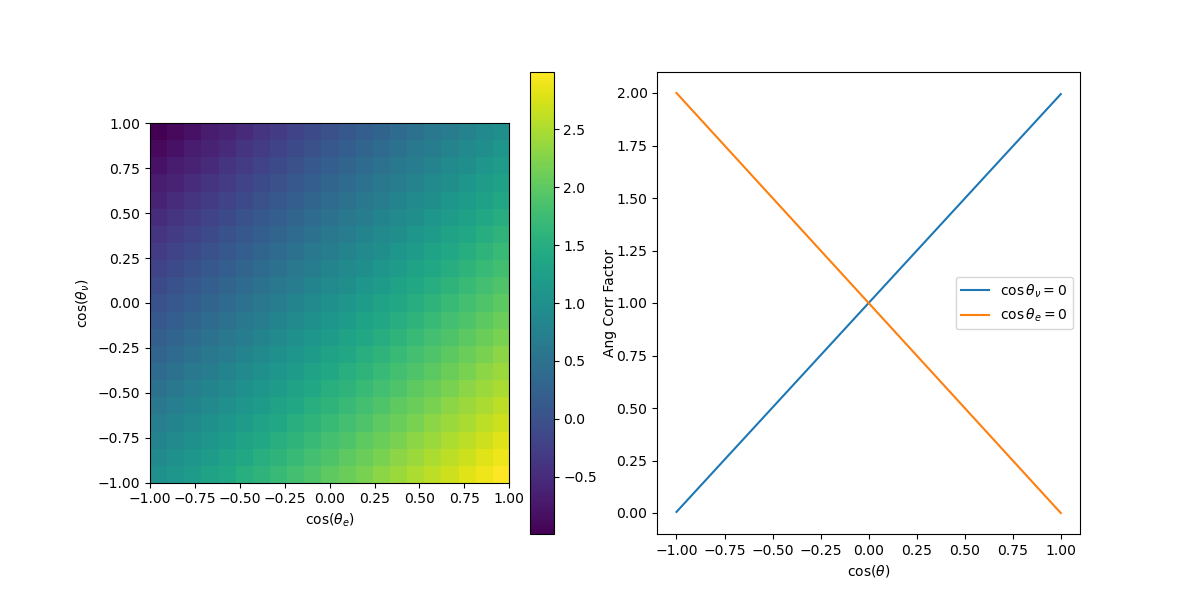
\includegraphics[width=0.8\paperwidth]{plots/posA_negB_hiE.png}
		\caption{(Right) Values of the angular correlation Factor with $A = 1$, $B = -1$, $E = 5000$ keV and rest of variables 0. Maximum = 2.99476, Minimum = -0.99476 (Left) 1D projections at any $\phi$, and either $z_e = 0$ (orange, m = 1) or $z_\nu = 0$ (blue, m = -0.9948)}	
	\end{figure}
\end{frame}
\begin{frame}{Note of Concern}
	\begin{itemize}
		\item Negative values for the angular correlation factor found in the tests. Concern for Montecarlo procedure.
		\item Possible in real simulations? Example from values in previous test:
		Gamov-Teller, $C_A = C_A' = C$, ($C_V, C_V'$ irrelevant), $\xi=2C|M_{GT}|^2$, $|A| = |B| = |\lambda_{J_i,J_f}|$ 
		$$|A| = |B| = \frac{2}{\xi}|M_{GT}|^2|\lambda_{J_i,J_f}||Re(C_A\overline{C_A'})|$$
		\item $|\lambda_{J_i,J_f}| = 1$, negative values can be found with certainity, $|\lambda_{J_i,J_f}| > 0.5$ negative values are posible depending on energy

	\end{itemize}
\end{frame}
\begin{frame}
	\begin{figure}
		\centering
		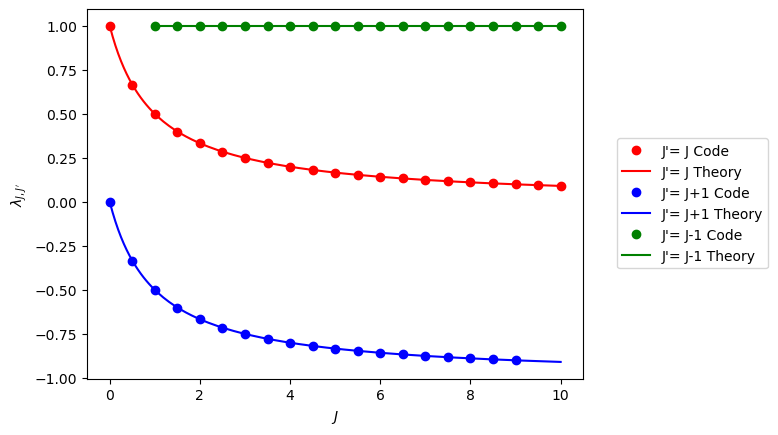
\includegraphics[height=0.5\paperheight]{plots/lambda_test_result.png}
	\end{figure}
	 Hope: Still need to consider $a$, which equals 
	 $$a = -\frac{|M_{GT}|^2(|C_A|^2+|C_A'|^2)}{3\xi}=-\frac13$$. 
	 Spoiler: situation worse ($A=-B$)
\end{frame}
\begin{frame}{Two variables: a and B}
	Since term proportional to a depends on E, we can consider different ratios by either:
	\begin{itemize}
		\item Fixing $a = B = 1$ and modifying the energy (first 3 plots)
		\item Same as before, but now $B = -1$ (last 2)
		\item Fixing $B = 1$ and $E \gg m_e \rightarrow \beta_e \approx 1$ and modifying $a > B$
	\end{itemize}
	
	We recall
	
	$$F = 1 + a\beta_e(z_ez_\nu + \sqrt{1-z^2_e}\sqrt{1-z^2_\nu}\cos \phi) + Bz_\nu$$
	
	Maxima and minima with $z_e=\pm1,z_\nu \pm1 \rightarrow \boldsymbol{p_e} \parallel \boldsymbol{p_\nu} \parallel \boldsymbol{J}$  
	
\end{frame}
\begin{frame}{Two variables: a and B}{Low Energy}
	\begin{figure}
		\centering
		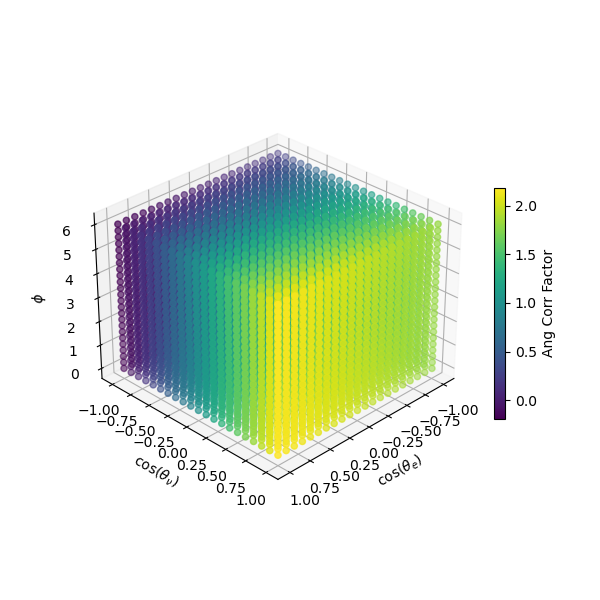
\includegraphics[width=0.4\paperwidth]{plots/posa_posB_lowE_3D}
		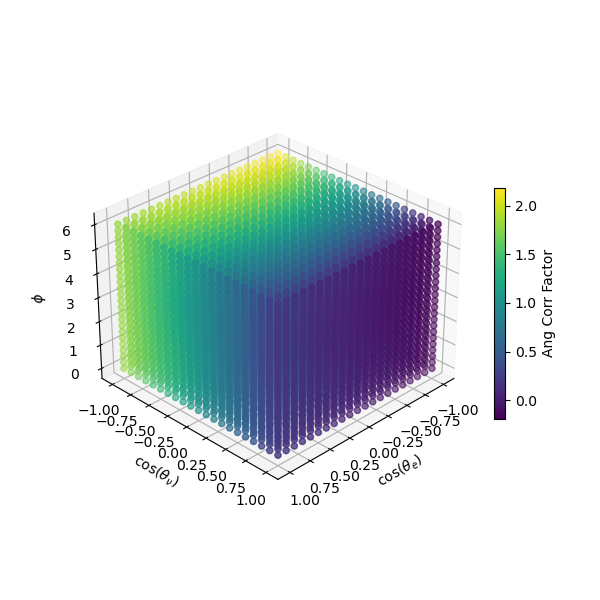
\includegraphics[width=0.4\paperwidth]{plots/posa_negB_lowE_3D}
		\caption{Values of the angular correlation Factor with (Right) a = 1, B = 1 and (Left) a = 1, B = -1; with E = 520 keV and rest of variables 0 for both.}
	\end{figure}
\end{frame}
\begin{frame}{Two variables: a and B}{High Energy}
	\begin{figure}
		\centering
		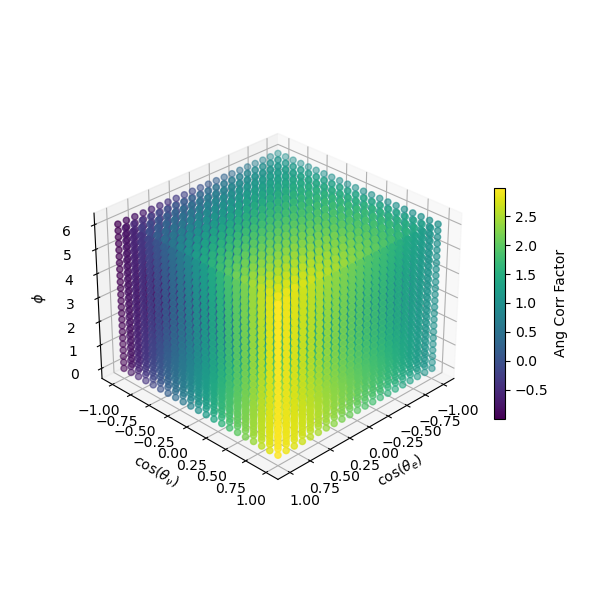
\includegraphics[width=0.4\paperwidth]{plots/posa_posB_hiE_3D}
		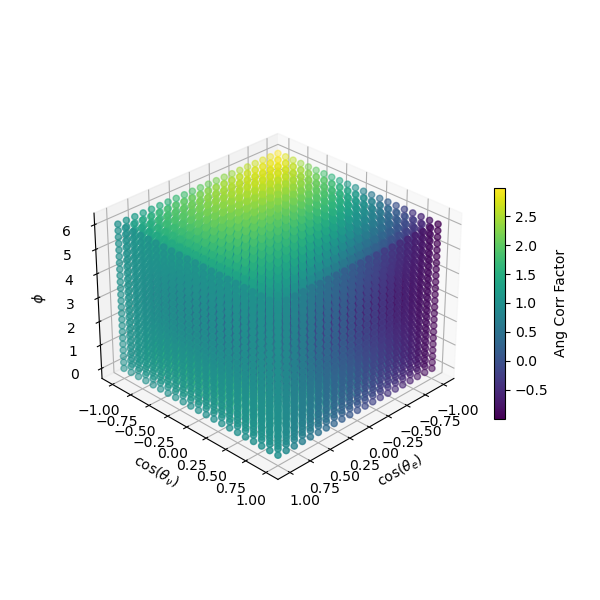
\includegraphics[width=0.4\paperwidth]{plots/posa_negB_hiE_3D}
		\caption{Values of the angular correlation Factor with (Right) a = 1, B = 1 and (Left) a = 1, B = -1; with E = 5000 keV and rest of variables 0 for both.}
	\end{figure}
\end{frame}
\begin{frame}{Two variables: a and B}{More Ratios}
	\begin{figure}
		\centering
		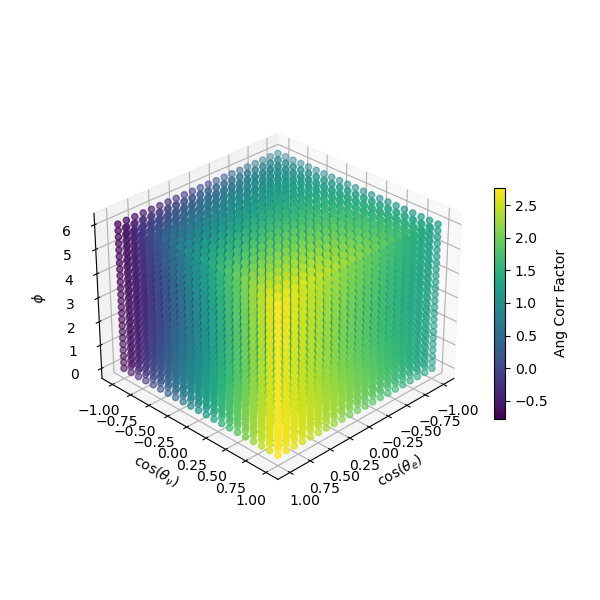
\includegraphics[width=0.4\paperwidth]{plots/posa_posB_medE_3D}
		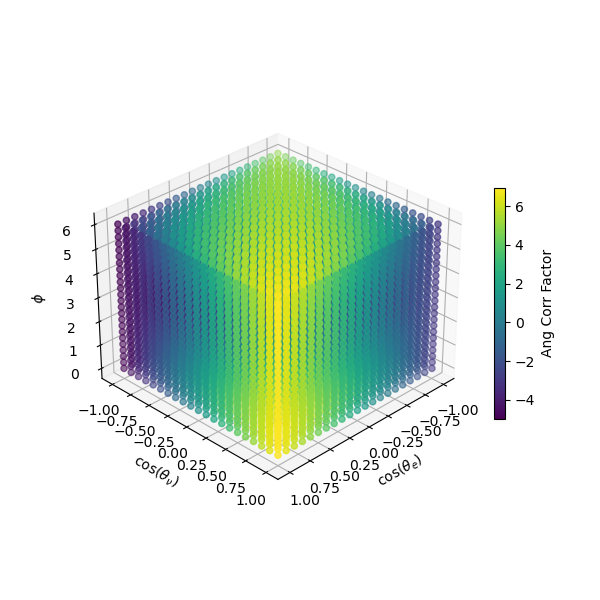
\includegraphics[width=0.4\paperwidth]{plots/posa_posB_vhia_3D}
		\caption{Values of the angular correlation Factor with (Right) a = 1, B = 1, E = 800 keV and (Left) a = 5, B = 1, E = 5000 keV; with the rest of variables 0 for both.}
	\end{figure}
\end{frame}
\begin{frame}{Two variables: a and B}{Maximum and Minimum}
	\begin{figure}
		\centering
		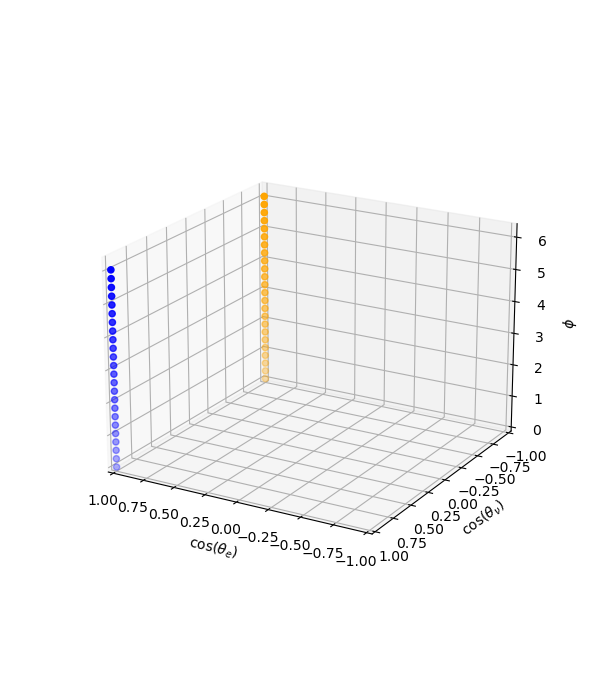
\includegraphics[width=0.4\paperwidth]{plots/posa_posB_hiE_max_min}
		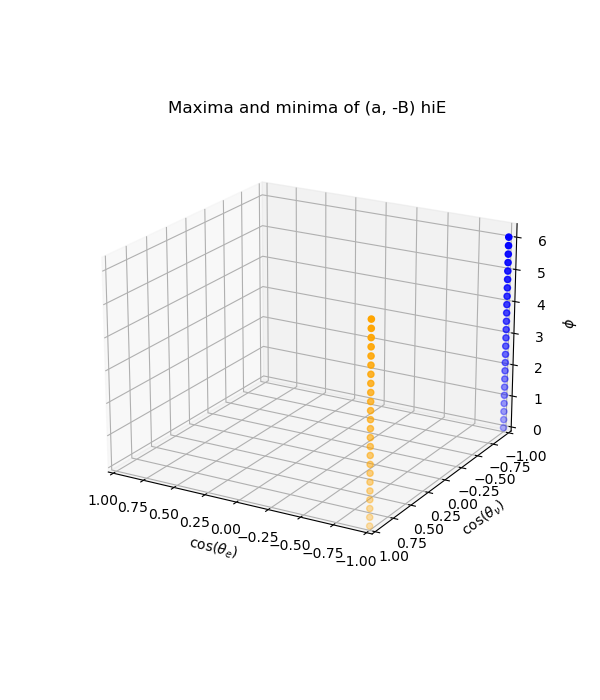
\includegraphics[width=0.4\paperwidth]{plots/posa_negB_hiE_max_min}
		\caption{Location of maximum (blue, value = 2.99476) and minimum (orange, value = -0.99476) for (Right) a = B = 1, E = 5000 keV and (Left) a = 1, B = -1, E = 5000 keV}
	\end{figure}
\end{frame}
\begin{frame}{Two variables: a and A}
	Since both terms proportional to a depends on E, we can consider only consider different ratios by changing one ($A$), while leaving the other ($a$) fixed. For convenience $E \gg m_e$.

	$$F = 1 + \beta_e(a (z_ez_\nu + \sqrt{1-z^2_e}\sqrt{1-z^2_\nu}\cos \phi) + Az_e)$$
	
	Maximum and minimum with $z_e=\pm1,z_\nu \pm1 \rightarrow \boldsymbol{p_e} \parallel \boldsymbol{p_\nu} \parallel \boldsymbol{J}$  
	
\end{frame}
\begin{frame}{Two variables: a and A}{$|A|\ll a$}
	\begin{figure}
		\centering
		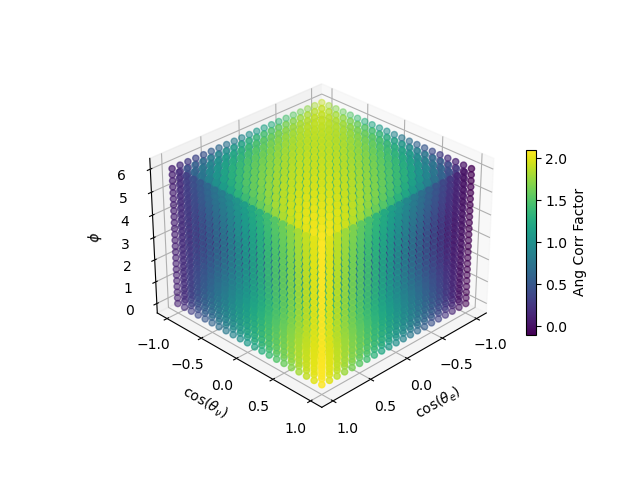
\includegraphics[width=0.4\paperwidth]{plots/posa_xsposA_3D}
		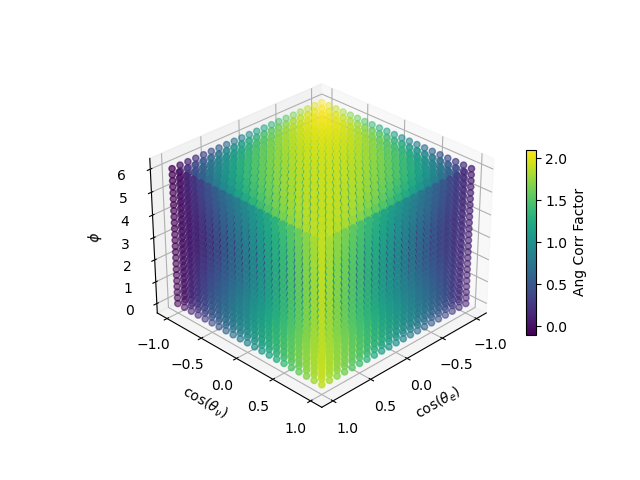
\includegraphics[width=0.4\paperwidth]{plots/posa_xsnegA_3D}
		\caption{Values of the angular correlation Factor with (Right) a = 1, A = 0.1 and (Left) a = 1, A = -0.1, with E = 100000 keV and rest of variables 0 for both.}
	\end{figure}
\end{frame}
\begin{frame}{Two variables: a and A}{$|A|= a$}
	\begin{figure}
		\centering
		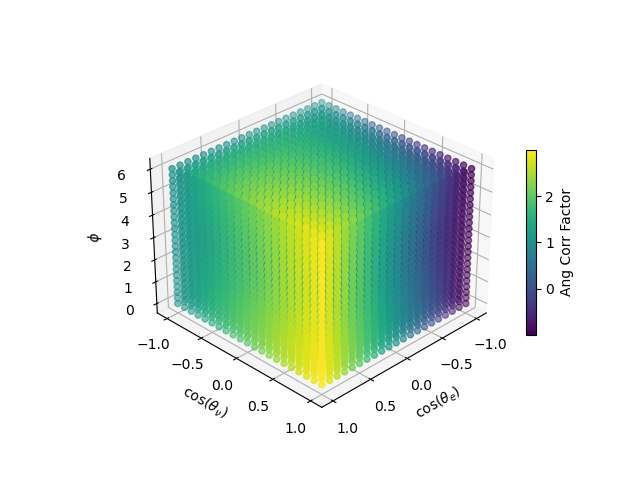
\includegraphics[width=0.4\paperwidth]{plots/posa_eqposA_3D}
		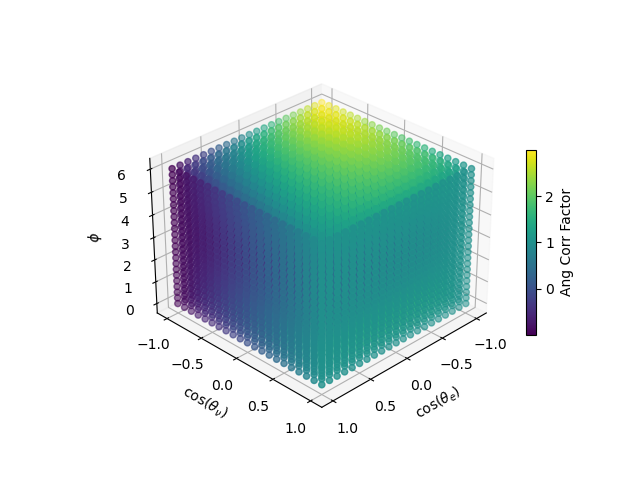
\includegraphics[width=0.4\paperwidth]{plots/posa_eqnegA_3D}
		\caption{Values of the angular correlation Factor with (Right) a = 1, A = 1 and (Left) a = 1, A = -1, with E = 100000 keV and rest of variables 0 for both.}
	\end{figure}
\end{frame}
\begin{frame}{Two variables: a and A}{$|A|\gg a$}
	\begin{figure}
		\centering
		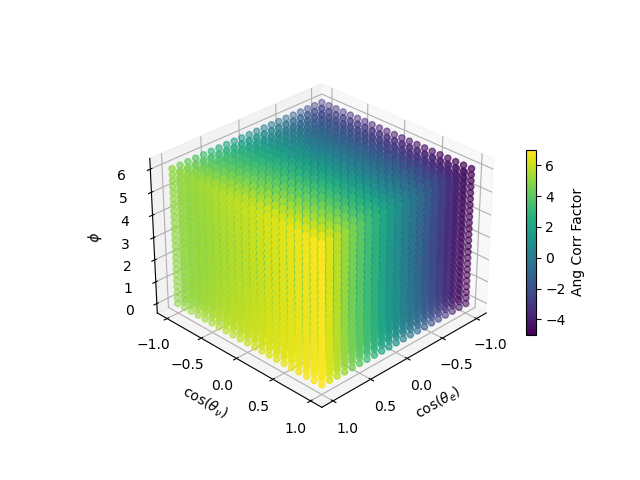
\includegraphics[width=0.4\paperwidth]{plots/posa_xlposA_3D}
		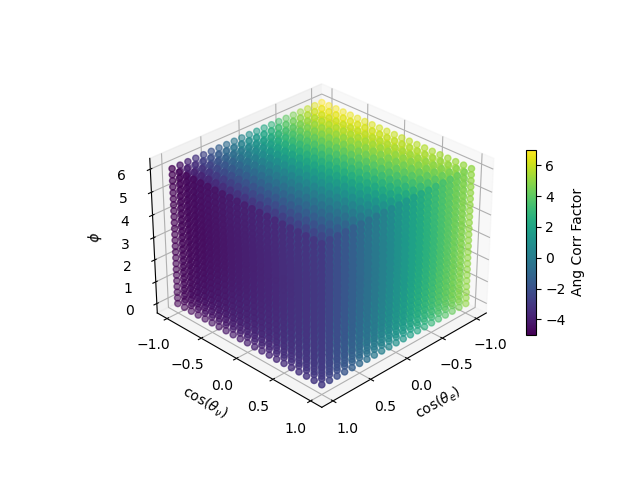
\includegraphics[width=0.4\paperwidth]{plots/posa_xlnegA_3D}
		\caption{Values of the angular correlation Factor with (Right) a = 1, A = 5 and (Left) a = 1, A = -5, with E = 100000 keV and rest of variables 0 for both.}

	\end{figure}
\end{frame}
\begin{frame}{Two variables: a and A}{Maximum and Minimum}
	\begin{figure}
		\centering
		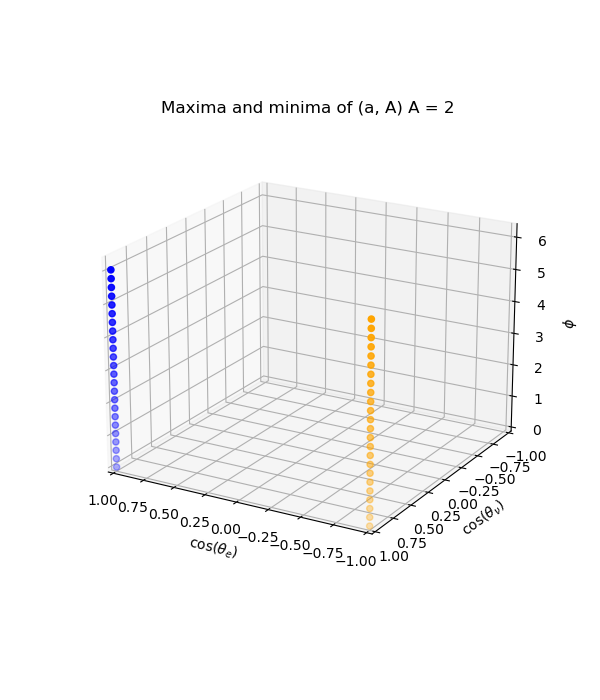
\includegraphics[width=0.4\paperwidth]{plots/posa_eqposA_max_min}
		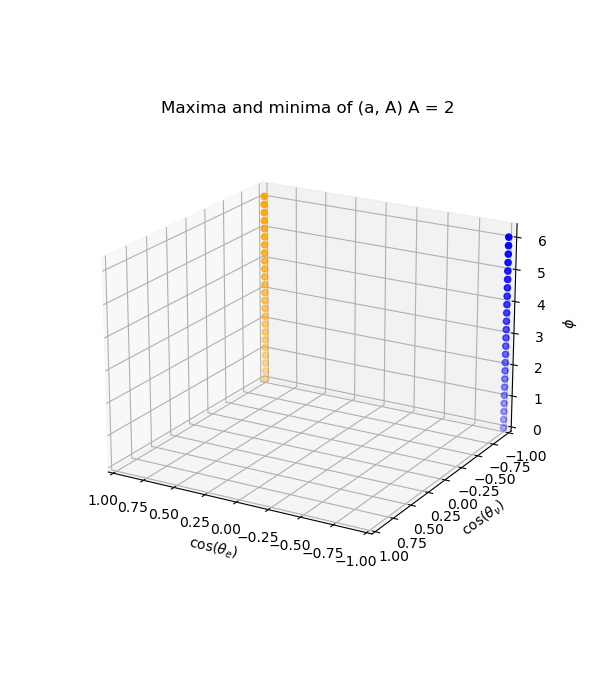
\includegraphics[width=0.4\paperwidth]{plots/posa_eqnegA_max_min}
		\caption{Location of maximum (blue, value = 2.99997) and minimum (orange, value = -0.99997) for (Right) a = B = 1, E = 5000 keV and (Left) a = 1, B = -1, E = 5000 keV}
	\end{figure}
\end{frame}
\begin{frame}{Two variables: B and D}
	Since term proportional to a depends on E, we can consider different ratios by either:
	\begin{itemize}
		\item Fixing $B = D = 1$ and modifying the energy
		\item Same as before, but now $B = -1$
		\item Fixing $B = 1$ and $E \gg m_e \rightarrow \beta_e \approx 1$ and modifying $a > B$
	\end{itemize}
	
	We recall
	
	$$F = 1 + D\beta_e\sqrt{1-z^2_e}\sqrt{1-z^2_\nu}\sin \phi + Bz_\nu$$
	
	Maxima and minima no longer at $z_e=\pm1,z_\nu \pm1$. In fact, expect $z_e = 0$, $\phi = \pm\pi/2$. Additionally, at the maximum:
	
	$$z_\nu = \frac B{\sqrt{D^2+B^2}}$$
	$$F = 1 + \sqrt{D^2+B^2}$$    

\end{frame}
\begin{frame}{Two variables: B and D}{3D examples}
	\begin{figure}
		\centering
		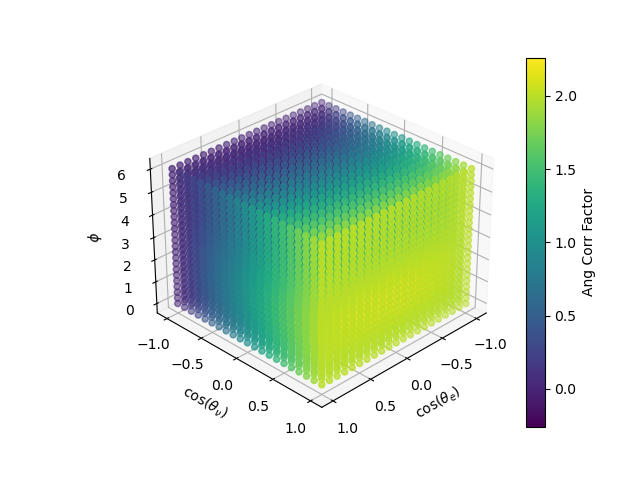
\includegraphics[width=0.4\paperwidth]{plots/posD_posB_medE_3D}
		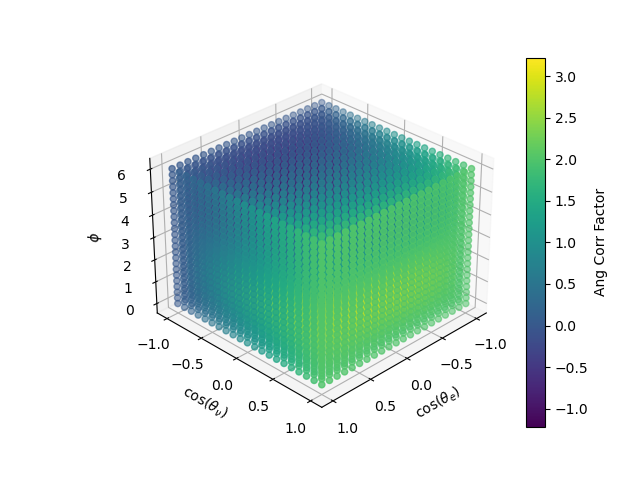
\includegraphics[width=0.4\paperwidth]{plots/posD_posB_hiD_3D}
		\caption{Values of the angular correlation Factor with (Right) D = 1, B = 1, E = 800 keV and (Left) D = 2, B = 1, E = 5000 keV, with the rest of variables 0 for both.}
	\end{figure}
	Image difficult to treat: consider only properties of the extrema.
\end{frame}
\begin{frame}{Two variables: B and D}{Low Energy}
	\begin{figure}
		\centering
		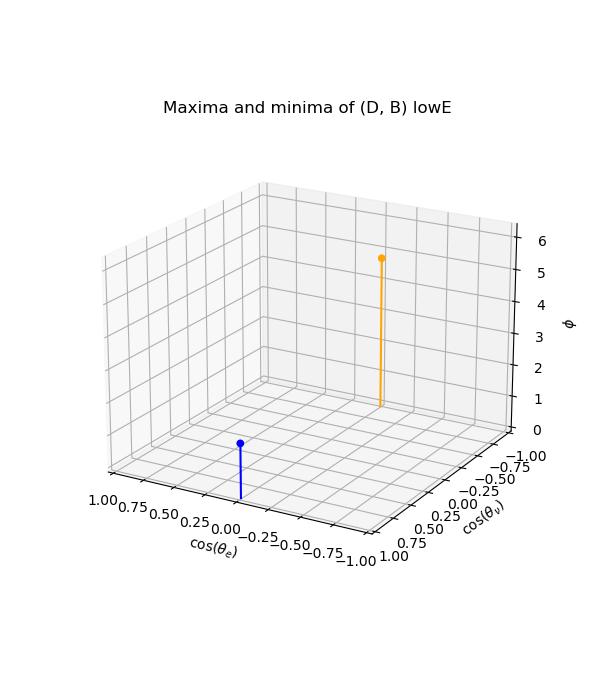
\includegraphics[width=0.4\paperwidth]{plots/posD_posB_lowE_max_min}
		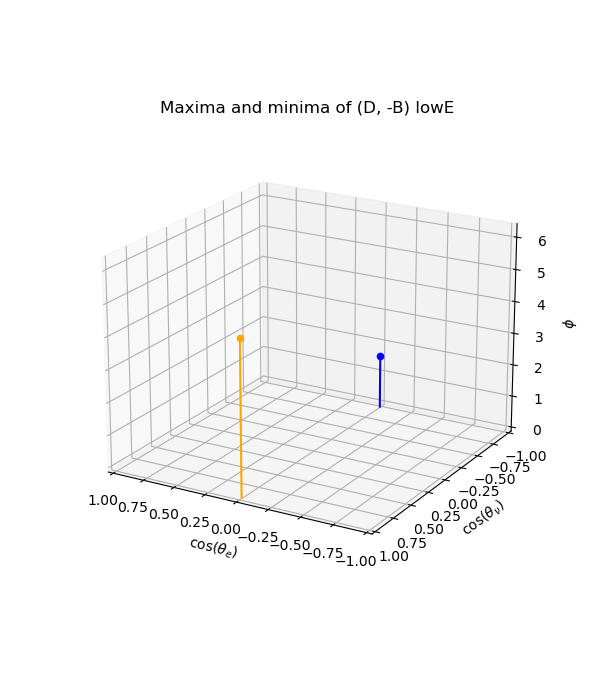
\includegraphics[width=0.4\paperwidth]{plots/posD_negB_lowE_max_min}
		\caption{Location of maximum (blue) and minimum (orange) for (Right) D = B = 1 (Left) D = 1, B = -1, both at E = 520 keV}
	\end{figure}
\end{frame}
\begin{frame}{Two variables: B and D}{High Energy}
	\begin{figure}
		\centering
		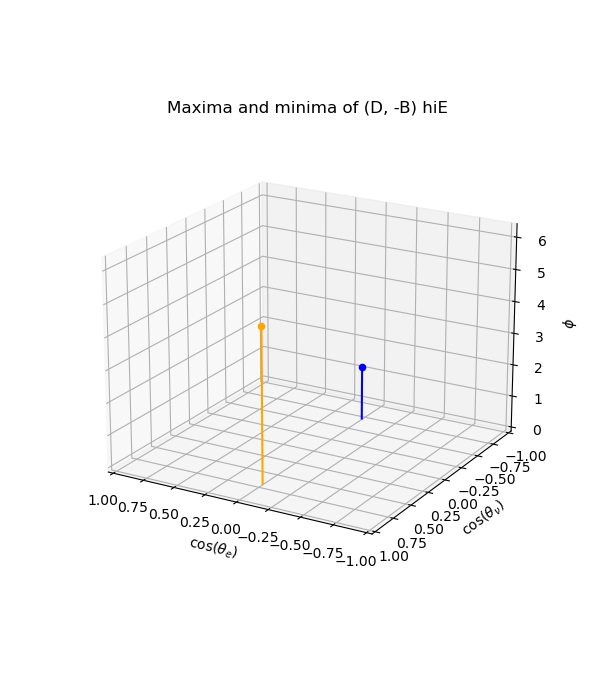
\includegraphics[width=0.4\paperwidth]{plots/posD_negB_hiE_max_min}
		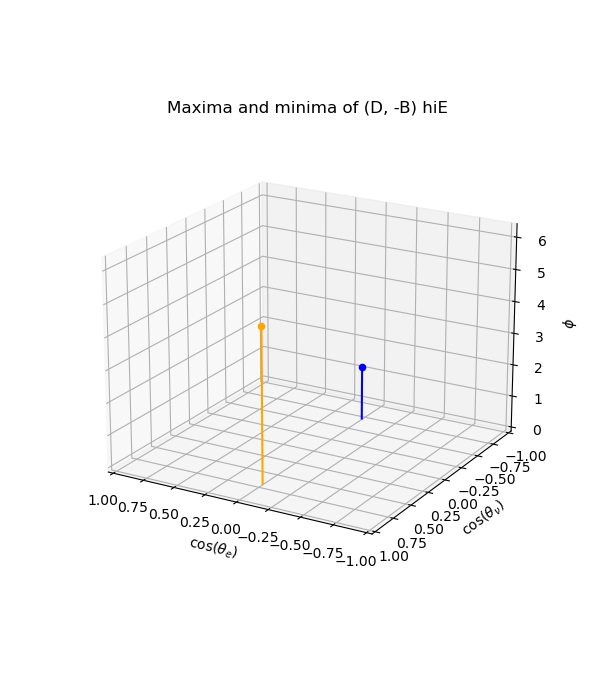
\includegraphics[width=0.4\paperwidth]{plots/posD_negB_hiE_max_min}
		\caption{Location of maximum (blue) and minimum (orange) for (Right) D = B = 1 and (Left) D = 1, B = -1, both at E = 5000 keV}
	\end{figure}
\end{frame}
\begin{frame}{Two variables: B and D}{More Ratios}
	\begin{figure}
		\centering
		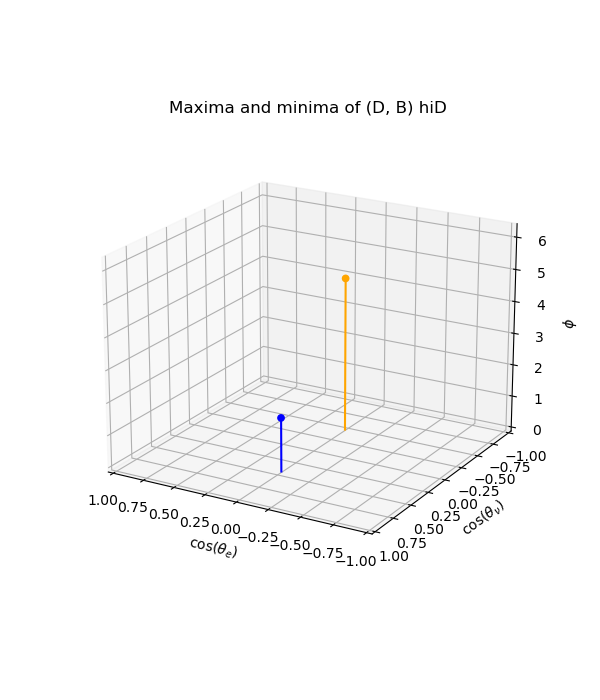
\includegraphics[width=0.4\paperwidth]{plots/posD_posB_hiD_max_min}
		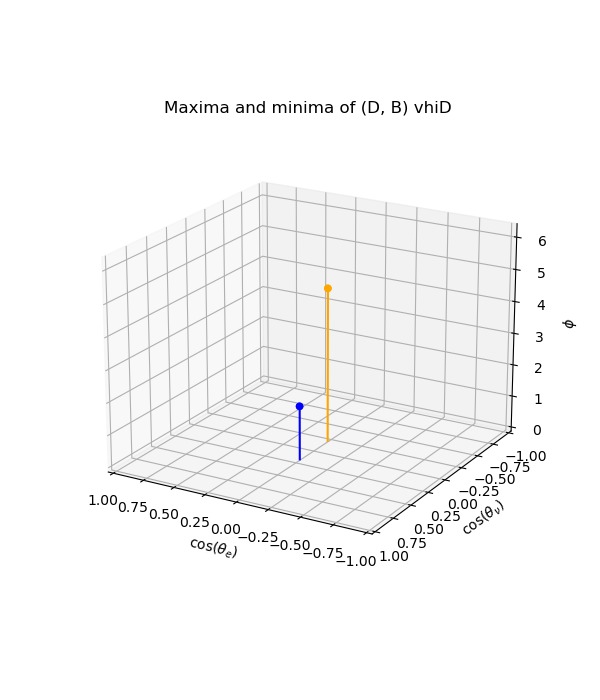
\includegraphics[width=0.4\paperwidth]{plots/posD_posB_vhiD_max_min}
		\caption{Location of maximum (blue) and minimum (orange) for (Right) D = 2, B = 1, E = 5000 keV and (Left) D = 5, B = 1, E = 5000 keV}
	\end{figure}
\end{frame}
\begin{frame}{Two variables: B and D}{Behaviour of maximum}
	Considering now only cases with $B > 0$:
	\begin{figure}
		\centering
		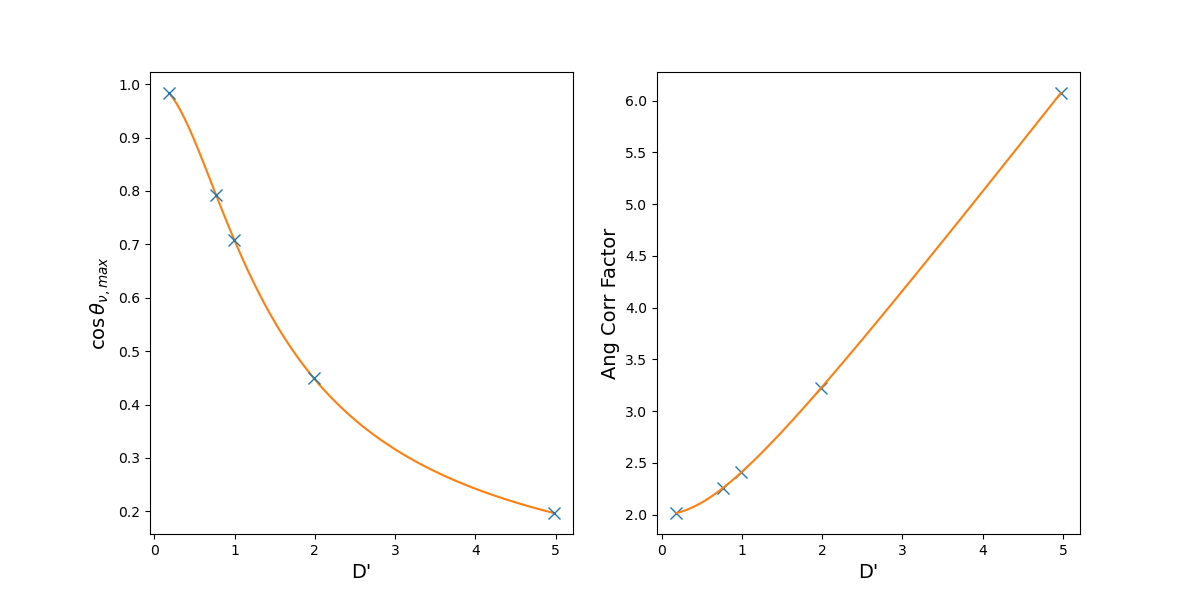
\includegraphics[width=0.8\paperwidth]{plots/BD_max_behaviour}
		\caption{Behaviour of the $z_\nu$ coordinate for the maximum and the maximum value of the angular correlation factor for diferent values of D}
	\end{figure}
\end{frame}
\begin{frame}{Two variables: A and D}
	Since both terms proportional to a depends on E, we can consider only consider different ratios by changing one ($A$), while leaving the other ($D$) fixed. For convenience $E \gg m_e$.

	$$F = 1 + D\beta_e\sqrt{1-z^2_e}\sqrt{1-z^2_\nu}\sin \phi + A\beta_ez_e$$
	
	Maxima and minima no longer at $z_e=\pm1,z_\nu \pm1$. In fact, expect $z_\nu = 0$, $\phi = \pm\pi/2$. Additionally, at the maximum:
	
	$$z_e = \frac A{\sqrt{D^2+A^2}}$$
	$$F = 1 + \sqrt{D^2+A^2}$$    

	We look directly at the properties of the extrema.
\end{frame}
\begin{frame}{Two variables: A and D}{$|A|\ll D$}
	\begin{figure}
		\centering
		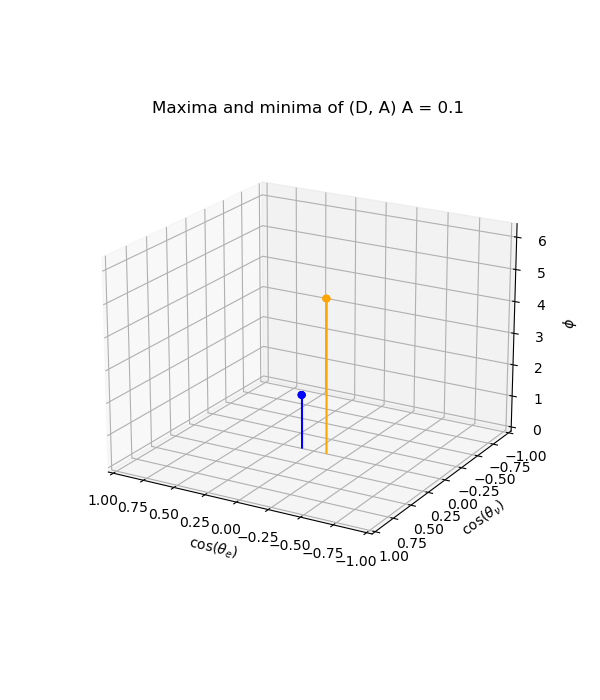
\includegraphics[width=0.4\paperwidth]{plots/posD_xsposA_max_min}
		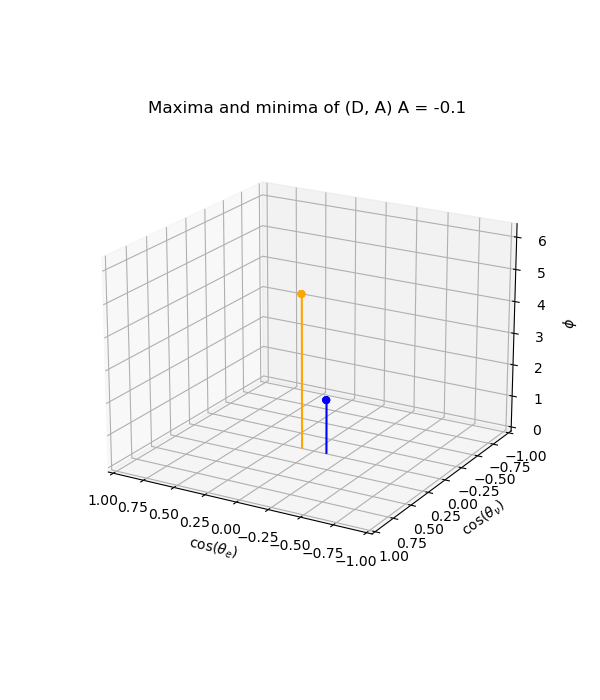
\includegraphics[width=0.4\paperwidth]{plots/posD_xsnegA_max_min}
		\caption{Positions of the maximum and minimum with Factor with (Right) D = 1, A = 0.1 and (Left) D = 1, A = -0.1, with E = 100000 keV and rest of variables 0 for both.}
	\end{figure}
\end{frame}
\begin{frame}{Two variables: A and D}{$|A|= D$}
	\begin{figure}
		\centering
		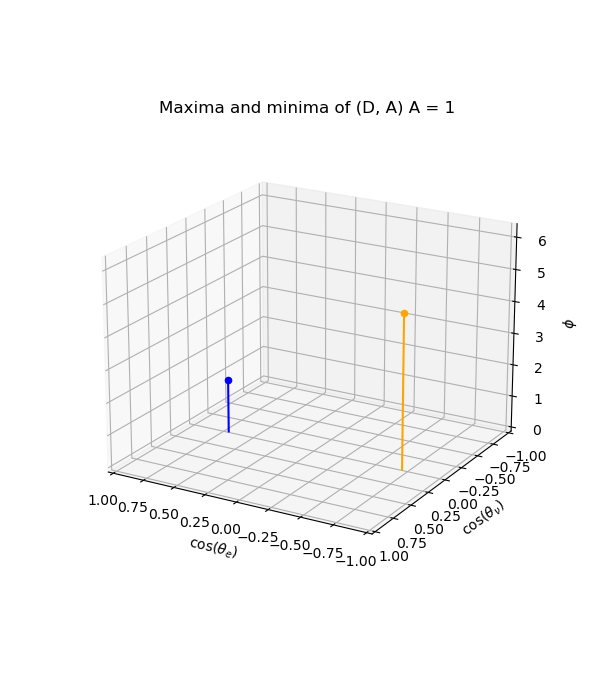
\includegraphics[width=0.4\paperwidth]{plots/posD_eqposA_max_min}
		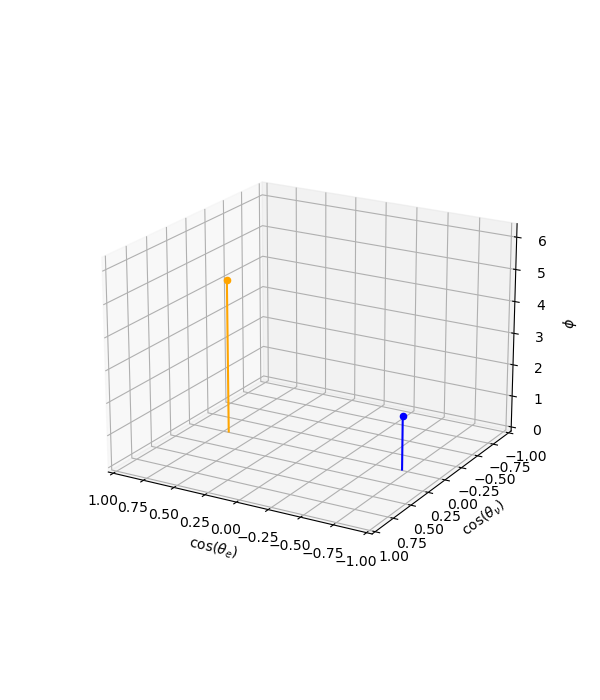
\includegraphics[width=0.4\paperwidth]{plots/posD_eqnegA_max_min}
		\caption{Positions of the maximum and minimum with with (Right) D = 1, A = 1 and (Left) D = 1, A = -1, with E = 100000 keV and rest of variables 0 for both.}
	\end{figure}
\end{frame}
\begin{frame}{Two variables: A and D}{$|A|\gg D$}
	\begin{figure}
		\centering
		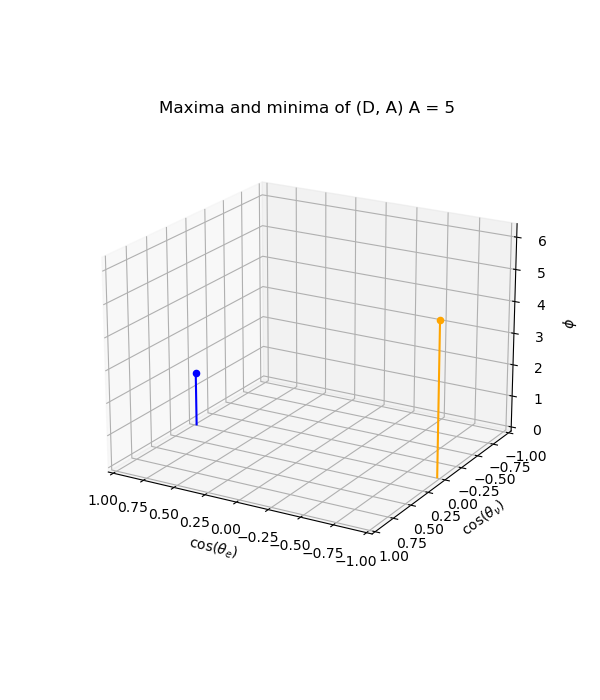
\includegraphics[width=0.4\paperwidth]{plots/posD_xlposA_max_min}
		\includegraphics[width=0.4\paperwidth]{plots/posD_xlposA_max_min}
		\caption{Positions of the maximum and minimum with (Right) D = 1, A = 5 and (Left) D = 1, A = -5, with E = 100000 keV and rest of variables 0 for both.}
	\end{figure}
\end{frame}
\begin{frame}{Two variables: A and D}{Behaviour of maximum}
\begin{figure}
	\centering
	\includegraphics[width=0.8\paperwidth]{plots/AD_max_behaviour}
	\caption{Behaviour of the $z_\nu$ coordinate for the maximum and the maximum value of the angular correlation factor for diferent values of A}
\end{figure}
\end{frame}
\begin{frame}{Two variables: a and D}
	Since both terms proportional to a depends on E, we can consider only consider different ratios by changing one ($D$), while leaving the other ($a$) fixed. For convenience $E \gg m_e$.
	
	$$F = 1 + \beta_e(a (z_ez_\nu + \sqrt{1-z^2_e}\sqrt{1-z^2_\nu}\cos \phi) + D\sqrt{1-z^2_e}\sqrt{1-z^2_\nu}\sin \phi)$$
	
	Maxima and minima no longer at $z_e=\pm1,z_\nu \pm1$. In fact, expect $z_\nu = 0$, $z_e = 0$. Additionally, at the maximum:
	
	$$\tan\phi = \frac Da$$
	$$F = 1 + \sqrt{D^2+a^2}$$    
	
	We look directly at the properties of the extrema.
\end{frame}
\begin{frame}{Two variables: a and D}{$|D|\ll a$}
	\begin{figure}
		\centering
		\includegraphics[width=0.4\paperwidth]{plots/posa_xsposD_max_min}
		\includegraphics[width=0.4\paperwidth]{plots/posa_xsnegD_max_min}
		\caption{Positions of the maximum and minimum with Factor with (Right) a = 1, D = 0.25 and (Left) a = 1, D = -0.25, with E = 100000 keV and rest of variables 0 for both.}
	\end{figure}
\end{frame}
\begin{frame}{Two variables: a and D}{$|D|= a$}
	\begin{figure}
		\centering
		\includegraphics[width=0.4\paperwidth]{plots/posa_eqposD_max_min}
		\includegraphics[width=0.4\paperwidth]{plots/posa_eqnegD_max_min}
		\caption{Positions of the maximum and minimum with with (Right) a = 1, D = 1 and (Left) a = 1, D = -1, with E = 100000 keV and rest of variables 0 for both.}
	\end{figure}
\end{frame}
\begin{frame}{Two variables: a and D}{$|D|\gg a$}
	\begin{figure}
		\centering
		\includegraphics[width=0.4\paperwidth]{plots/posa_xlposD_max_min}
		\includegraphics[width=0.4\paperwidth]{plots/posa_xlnegD_max_min}
		\caption{Positions of the maximum and minimum with (Right) a = 1, D = 4 and (Left) a = 1, D = -4, with E = 100000 keV and rest of variables 0 for both.}
	\end{figure}
\end{frame}
\begin{frame}{Two variables: a and D}{Behaviour of maximum}
	\begin{figure}
		\centering
		\includegraphics[width=0.8\paperwidth]{plots/aD_max_behaviour}
		\caption{Behaviour of the $\phi$ coordinate for the maximum and the maximum value of the angular correlation factor for diferent values of A}
	\end{figure}
\end{frame}

\begin{frame}{Three variables: a, A, B}
	We come back to the case we hinted at before, that is compatible with all Gamov-Teller decays within the Standard Model framework.
	
	Gamov-Teller, $C_A = C_A' = C$, ($C_V, C_V'$ irrelevant), $\xi=2C|M_{GT}|^2$, $|A| = |B| = |\lambda_{J_i,J_f}|$ 
	$$|A| = |B| = \frac{2}{\xi}|M_{GT}|^2|\lambda_{J_i,J_f}||Re(C_A\overline{C_A'})| = |\lambda_{J_i,J_f}|$$
	$$a$$
	
	We consider different values of $|A|$, particularly with $|A| > 0.5$, and a range of electron energies from very low to very high.
	
\end{frame}
\begin{frame}
	\begin{figure}
	\centering
	\includegraphics[width=0.8\paperwidth]{plots/aAB_gt_current_physics}
	\caption{Values of the maximum and minimum for different combinations of $|A|$ and E. In red, values that are negative}
	\end{figure}
\end{frame}

\end{document}


